\chapter{Plitvice Workflow}

\section{Terminologia e convenzioni}
Un workflow si compone di una serie di stati collegati l'uno a l'altro tramite passaggi detti transizioni. Il modo più utile per rappresentare un workflow è quello di utilizzare un grafo come quello seguente:

\begin{figure}[h!]
  \centering
    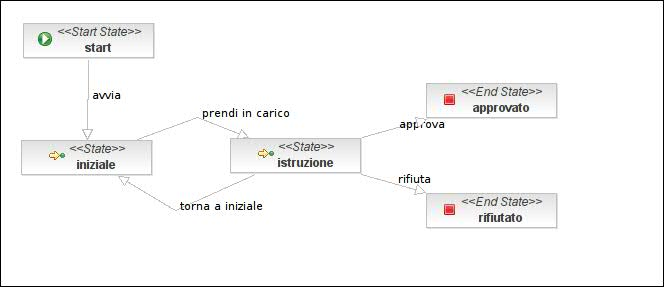
\includegraphics[scale=0.5]{workflow} 
  \caption[workflow]{Grafico di un workflow \label{fig:workflow}}
\end{figure}

Nel flusso di esempio sono presenti cinque stati: \textit{start}, \textit{iniziale}, \textit{istruzione}, \textit{approvato} e \textit{rifiutato}.  Nella definizione di un nuovo flusso conviene rammentarsi di aderire ad alcune convenizioni stabilite da Plitvice kit: ad esempio conviene di utilizzare come nomi degli stati  
\begin{inparaenum}[\itshape a\upshape)]
\item  solo caratteri minuscoli e possibilemente \item preferire gli aggettivi ai sostantivi. 
Ogni workflow deve necessariamente \item iniziare  con lo stato \textit{start} che deve prevedere  \item un'unica transizione denominata avvia.
Tornando all'esempio le altre transizioni sono \textit{prendi in carico}, \textit{torna a iniziale}, \textit{approva} e \textit{rifiuta}; da notare la convenzione di utilizzare \item dei verbi in modo imperativo per definire le transizioni. 
Infine alcuni stati sono detti terminali perché una volta raggiunti non è più possibile lasciarli (nell'esempio \textit{approvato} e \textit{rifiutato}).
\end{inparaenum}


\section{Tabella di marcia}
Le applicazioni Regola kit possono essere configurate per la gestione di workflow semplicemente aggiungendo una dipendenza al modulo \textit{plitvice-workflow}. Predisporre invece un proprio gestore di flussi richiede diverse operazioni:

\begin{itemize*}
\item definire un Workflow
\item creare un WorkflowRepository
\item definire un Ruolo con i relativi Diritti
\item progettare una classe di Visibilità
\item creare un AuthenticationManager
\item progettare il documento
\item progettare la classe WorkflowManager
\item progettate la classe WorkflowActions
\end{itemize*}

In effetti sembrano parecchie ma in realtà sono piuttosto veloci da approntare perché Plitvice kit fornisce tutte le classi di basi necessarie ad un'applicazione reale: ad esempio sono già previsti i supporti per i WorkflowRepository su database o in memoria tramite mock.
Nel corso della presentazione verranno toccati tutti i punti dell'elenco e si provvederà a realizzare un esempio concreto per la gestione di un Workflow denominato \textit{accordo} in grado di gestire un documento di tipo Accordo.

\section{Workflow}
Plitvice kit utilizza JBoos jBPM internamente per la gestione dei Workflow. La definizione di un Workflow avviene quindi mediante un file XML che raccoglie gli stati e le transizioni. Per chi utilizza Eclipse è disponibile un comodo plug in visuale che può essere di un qualche aiuto nella progettazione del workflow. Affinché la definizione sia fruibile da Plitvice kit è necessario che si attenga alle seguenti convenzioni:

\begin{itemize*}
\item il file xml contenente la definizione deve essere salvato nella posizione  src/main/resources/workflows/nomeflusso/processdefinition.xml

\item il nodo iniziale di ogni flusso deve chiamarsi \textit{start} 

\item dal nodo iniziale deve uscire solo una transizione denominata \textit{avvia}

\item ogni transizione che prevede una modifica di database deve essere associata ad un'azione gestita dalla classe PersistenceAction come nel frammento di definizione seguente:
\begin{xml}
<state name="iniziale">
    <transition to="istruzione" name="prendi in carico">
      <action class="it.kion.plitvice.workflow.service.impl.PersistenceAction"></action>
    </transition>
  </state>
\end{xml}

\item i nomi degli stati devono contenere solo caratteri minuscoli e possibilmente essere espressi medianti aggettivi (tipo iniziale, approvato, ecc.)

\item i nome delle transizioni devono contenere solo caratteri minuscoli e possibilmente essere espressi mediante verbi nel modo imperativo (tipo accetta, rifiuta, ecc.)

\end{itemize*}


\section{WorkflowRepository}
Un WorkflowRepository è un'entità di modello che consente di accedere a tutti i Workflow disponibili per l'applicazione in modo che i WorkflowManager possano, conoscendone solo il nome, accedere a tutte le proprietà di un flusso, compresa la definizione. 
Generalmente il repository si concretizza semplicemente in una tabella di database che elenchi i diversi workflow e ne raccolga gli attributi. Plitvice kit prevede una classe per gestire questa tabella,  WorkflowRepositoryHibernate.
Alternativamente, spesso impiegati per la fase di test, si può creare un repository in memoria popolato mediante configurazione di Spring (si veda ad esempio WorkflowRepositoryMock).

\section{Autorizzazioni}

L'autorizzazione su un workflow consiste nello stabilire se l'identità correntemente assunta dell'utente autenticato possa o meno segnalare una certa transizione oppure abbia i permessi per elencare i documenti in un certo stato. Lo schema delle autorizzazioni è quello definito nel modulo plitvice security che prevede il concetto di Ruolo a cui fa capo una collezione di diritti (Diritto); questi ultimi possono essere di natura applicativa oppure relativi ai workflow. Infine questi ultimi si distinguono per occuparsi degli stati oppure delle transizioni.

Gli elementi comuni ad ogni diritto sono un identificativo unico (un intero) ed un Ambito che rappresenta un partizionamento su base applicativa; ad esempio esiste l'ambito dei tirocini che raccoglie tutti i diritti relativi alla grande area della gestione dei tirocini. Inoltre tutti i diritti fanno riferimento ad un'Entità, ovvero un elemento del modello con un ciclo di vita ampio secondo i dettami del Domain Driven Development. L'elenco delle Entità è persistito su database e a ciascuna è assegnato un identificativo univoco. I diritti relativo a workflow contengono invece sempre l'indicazione del flusso.\footnote{Attualmente dato un workflow discende una ed una sola entità per cui basterebbe l'indicazione del flusso per risalire inequivocabilmente all'entità; comunque al momento in cui questo manuale è redatto, sia l'id dell'entità che il nome del flusso devono specificate in modo congruente.}

I diritti di workflow di tipo transazione prevedono la possibilità di segnalare una specifica transazione. Il default, ovvero in caso di assenza di uno specifico diritto, la transazione non può essere segnalata da nessuno.
I diritti di workflow di tipo stato consentono di elencare tutti i documenti che si trovino in quello stato. In assenza di un particolare diritto chiunque può richiedere l'elenco completo dei documenti per quel certo stato. Esiste comunque un meccanismo che consente anche ad identità che non avrebbero i diritti di accedere all'elenco dei documenti; si rimanda alla proprietà vincoloLettura di AutorizzazioneUtente e l'interfaccia Visibilità per dettagli in merito.

Le autorizzazioni sono abilitate o disabilitate tramite un aspetto di Spring; per attivarle  basta aggiungere le seguenti righe in un file di configurazione di bean:
\begin{xml}
<!-- Enable @AspectJ support -->
<aop:aspectj-autoproxy proxy-target-class="false" />
  
<bean class="it.kion.plitvice.autorizzazioni.WorkflowManagerAuthentication" >
   <property name="authentication" ref="authenticationManager" />
</bean>
\end{xml}

\section{Il documento}
Un workflow documentale è destinato alla gestione di un documento, ad esempio potrebbe rappresentare i passi necessari e le persone (o gli uffici) coinvolti nel processo ufficiale di produzione di una pratica. 
In questo contesto il termine documento si riferisce ad  una classe Java, in particolare  un'entità di modello applicativo per la quale è eventualmente stato definito un  Model Pattern di Regola kit. Nel corso di questo capitolo, come si è detto, presenteremo un esempio concreto il cui documento è  l'entità Accordo:

\begin{java}
package it.kion.plitvice.workflow.model;

import it.kion.plitvice.workflow.service.impl.AccordoWorkflowActions;
import it.kion.plitvice.workflow.service.impl.AccordoWorkflowActions.Stati;

import java.io.Serializable;

public class Accordo implements Serializable {

  private Stati stato = Stati.start;
  private Long id = null;
  
  public void setStato(Stati stato) {
    this.stato = stato;
  }

  public Stati getStato() {
    return stato;
  }

  public void setId(Long id) {
    this.id = id;
  }

  public Long getId() {
    return id;
  }
  
}
\end{java}

Durante la fase di progettazione del documento deve essere tenuta in considerazione la relazione forte che lega  il documento al workflow che lo gestisce; in qualsiasi momento del ciclo di vita del documento deve esistere un modo (un algoritmo)  che partendo da un'istanza del documento sappia determinare il workflow di riferimento unitamente allo stato in cui il workflow si trova.  In altri termini lo stato del workflow deve essere desumibile attraverso il documento stesso, o perché lo contiene direttamente  o perché contiene gli elementi per recuperare da una database lo stato del flusso. 
Nel nostro semplice esempio lo stato è del flusso è semplicemente una proprietà del documento.

Il WorkflowManager consentirà di effettuare delle selezioni dalla popolazione di tutti i documenti gestiti tramite flussi: sarà in particolare possibile ottenere l'elenco di tutti i documenti che si trovino in un certo stato oppure gestiti da un certo workflow. Per effettuare questo genere d'interrogazioni è stato esteso il meccanismo di ModelPattern con due annotazioni, @Stati e @Workflow.

\begin{java}

package it.kion.plitvice.workflow.dao;

import it.kion.plitvice.workflow.model.Workflow;
import it.kion.plitvice.workflow.pattern.Stati;

import org.regola.model.ModelPattern;

public class AccordoPattern extends ModelPattern {

  String[] inStati = new String[] {};
  private Workflow flusso;

  @Stati()
  public String[] getInStati() {
    return inStati;
  }

  public void setInStati(String[] inStati) {
    this.inStati = inStati;
  }
  
  @it.kion.plitvice.workflow.pattern.Workflow
  public Workflow getFlusso() {
    return flusso;
  }

  public void setFlusso(Workflow flusso) {
    this.flusso = flusso;
  }
  
}
\end{java}

Tanto per avere un'idea fin da subito del funzionamento del ModelPattern nel contesto dei workflow può risultare utile l'esempio seguente che richiede al gestore del flusso tutti i documenti che si trovino nello stato \textit{iniziale} mediante una chiamata al metodo elencoProcessiInStati. 

\begin{java}
AccordoPattern pattern = new AccordoPattern();
pattern.setInStati(new String[] { "iniziale" });
    
// recupero il documento gestito dal flusso
List<Accordo> accordi = 
 accordoManager.elencoProcessiInStati(pattern, autNicola);
\end{java}


Come si vede prima si imposta AccordoPattern con lo stato d'interesse (iniziale) e poi lo si passa al metodo elencoProcessiInStati


\section{WorkflowManager: funzionamento}
Nel livello di servizio, assieme agli altri Business Delegate, i Service Facade ed in generale tutte le classi che consentono di fruire del modello, trovano collocazione i WorkflowManager; si tratta di Manager nel senso indicato da Regola kit che offrono un'interfaccia comune per la gestione dei flussi di lavoro. 

\begin{java}
public interface WorkflowManager
<D extends Serializable, ID extends Serializable> 
extends GenericManager<D,ID> {

  List<D> elencoProcessiInStati(ModelPattern pattern, AutorizzazioniUtente utente);
  int countProcessiInStati(ModelPattern pattern, AutorizzazioniUtente utente);
  
  String segnala(D processo, String transizione,AutorizzazioniUtente utenti) throws ProcessoNonValidoException, TransizioneNonValidaException;
  
  String avviaFlusso(Workflow flusso,Object documentoIniziale,AutorizzazioniUtente utenti);
  String avviaFlusso(Object documentoIniziale,AutorizzazioniUtente utenti);

  List<String> transizioniDisponibili (D processo, AutorizzazioniUtente utente);

  public List<String> elencoStati(D processo);


  Workflow[] elencoFlussiGestiti();

}
\end{java}


Ogni WorkflowManager si occupa di un solo tipo di documento D (un entità serializzabile e persistibile su database) la cui chiave d'identificazione è del tipo ID. Ricordo che il tipo D (il documento) può essere associato ad uno o più workflow tutti gestiti dallo stesso WorkflowManager; per sapere quali sono i flussi di lavoro gestiti da un WorkflowManager bisogna invocare il metodo   elencoFlussiGestiti(). Non bisogna dimenticare che se la classe D del documento può essere gestita da diversi flussi la singola istanza è gestita solo da uno ed un solo flusso; ovvero se un'istanza inizia il suo percorso all'interno di un workflow non può abbandonarlo più. Da questo deriva che data istanza di D è possibile determinare in modo univoco il flusso che la gestisce ed in questo modo è utilizzata all'interno degli altri metodi di WorkflowManager. 
Un'altra considerazione generale riguarda il sistema di autorizzazione che verifica le credenziali dell'utente collegato prima di consentire l'elencazione di documenti in un certo stato oppure la segnalazione di una transizione; molti metodi di WorkflowManager richiedono il passaggio di un DTO chiamato AutorizzazioniUtente che consente di individuare con esattezza l'identità selezionata dall'utente corrente ed applicare i criteri di autorizzazione. Per maggiori dettagli si rimanda al modulo plitvice security.

Il primo metodo da invocare per avviare un nuovo servizio è avviaFlusso() al quale si può eventualmente passare un oggetto preliminare che contenga le informazioni necessarie per creare il documento da inserire nel flusso. Naturalmente documento e oggetto preliminare possono coincidere se lo si ritiene conveniente. Come si è visto data un'istanza di documento  è possibile risalire al flusso; nel momento che precede la creazione di un nuovo flusso però quell'istanza non esiste per cui è necessario specificare al  metodo avviaFlusso() quale workflow utilizzare tra quelli gestiti da uno specifico WorkflowManager. Se si omette questa indicazione sarà utilizzato il primo workflow tra quelli gestiti.

Una volta avviato un flusso è possibile elencare tutti i documenti che si trovino in un certo stato tramite il metodo  elencoProcessiInStati() passandogli come parametro un ModelPattern come indicato nel paragrafo precedente.

Avuto un documento in un certo stato è possibile sapere quali siano le transizioni che gli sono consentite dall'identità correntemente assunta tramite il metodo  transizioniDisponibili().

Infine per segnalare una transizione (cioè cambiare stato) si richiami il metodo  segnala().


\section{WorkflowManager: progettazione}

La creazione di un servizio di workflow si limita alla creazione di un'interfaccia che estenda WorkflowManager e nel darne un'implementazione di massima.

\begin{java}

public interface AccordoWorkflowManager 
 extends WorkflowManager<Accordo, Long> {
}

public class AccordoWorkflowManagerImpl 
extends WorkflowManagerImpl<Accordo, Long> 
implements AccordoWorkflowManager 
{

  public AccordoWorkflowManagerImpl(GenericDao<Accordo, Long> dao) {
    super(dao);
    setFlussiGestiti(new String[] { "accordo" });
  }

  @Override
  protected void addProcessVariable(ProcessInstance instance) {
    // TODO Auto-generated method stub
  }

  @Override
  public Workflow flowForDocument(Accordo documento) {
    return repository.findByName(flussiGestiti[0]);
  }
  
}

\end{java}


I metodi di cui occuparsi nell'implementazione sono il costruttore in cui specificare i workflow gestiti da questo WorkflowManager, nell'esempio solo uno di nome \textit{accordo} che per quando indicato nelle convenzioni relativi alle definizioni dei workflow deve trovarsi nella posizione src/main/resources/workflows/accordo/processdefinition.xml.
Il metodo flowForDocument() consente di individuare a quale flusso sia associato l'istanza del documento; nel nostro esempio ogni istanza è gestita da un solo workflow.
Infine addProcessVariable() consente di inserire delle variabili da utilizzare all'interno delle action durante le segnalazioni. Nell'esempio non è impiegato questo metodo.
Il file di definizione di Spring per le classi appena create deve assomigliare al seguente frammento:

\begin{xml}
<bean id="accordoActions" class="it.kion.plitvice.workflow.service.impl.AccordoWorkflowActions" >
  <property name="dao" ref="accordoDao" />
</bean>
  
<bean id="accordoManager" class="it.kion.plitvice.workflow.service.impl.AccordoWorkflowManagerImpl" >
   <constructor-arg>
      <ref bean="accordoDao"/>
    </constructor-arg>
        <property name="actions" ref="accordoActions" />
    <property name="repository" ref="workflowRepositoryMock" />
    <property name="visibilitaFactoryChain" ref="visibilitaFactoryChain" />
</bean>
\end{xml}

Come si può osservare le dipendenze di ogni WorkflowManager sono la classe di actions che si occupa come si vedrà di definire le logiche di persistenza, un elemento di modello chiamato repository che si occupa di fornire l'accesso a tutte le difinizioni dei workflow disponibili per l'applicazione ed infine una  visibilitaFactoryChain che è intimamente legata con i criteri di applicazione delle autorizzazioni per cui si rimanda alla documentazione del modulo plitvice security per i dettagli.

\section{WorkflowActions}

La persistenza del workflow (e del documento a cui si riferisce) può essere completamente personalizzata tramite la progettazione di una classe che estenda WorkflowActions; i metodi di questa classe saranno richiamati (internamente da WorkflowManager )  al momento di attraversare una transizione o quando è richiesto un elenco di documenti. 
Molto probabilmente la vostra classe di action avrà un dao di Regola kit tra le dipendenze e lo userà nei modi consueti finendo per assomigliare ad una versione complessa di quella presentata qui di seguito:

\begin{java}
public class AccordoWorkflowActions 
   extends WorkflowActions<Accordo> {
  
  public enum Stati {
    start, iniziale, istruzione, approvato, rifiutato
  };
  
  private AccordoDao dao;
  
  public List<Accordo> elencoProcessiInStati(Workflow flusso, String [] stati, ModelPattern p, AutorizzazioniUtente utente)
  {
    log.info("elencoProcessiInStati=");
    return getDao().find(p); 
  }
  
  public int countProcessiInStati(Workflow flusso, String [] stati, ModelPattern p, AutorizzazioniUtente utente) 
  {
    log.info("countProcessiInStati=");
    return getDao().count(p);
  }
  
    @Override
  @StatoCorrente()
  public String getStatoCorrente(Accordo documento)
  {
    return documento.getStato().toString();
  }
  
  @Override
  public String avviaFlusso(Object documentoIniziale, AutorizzazioniUtente utente) {
    log.info("avviaFlusso");
    
    Accordo accordo = new Accordo();
    
    accordo.setId(1l);
    accordo.setStato(Stati.iniziale);
    
    dao.save(accordo);
    
    return Stati.iniziale.toString();
  }
  
  @Transizione("prendi in carico")
  public void segnalaPrendiInCarico(Accordo documento, String transizione, AutorizzazioniUtente utente) {
    documento.setStato(Stati.istruzione);
    dao.save(documento);
  }

  @Transizione("torna a iniziale")
  public void segnalaTornaAIniziale(Accordo documento, String transizione, AutorizzazioniUtente utente) {
    documento.setStato(Stati.iniziale);
    dao.save(documento);
  }

  @Transizione("approva")
  public void segnalaApprova(Accordo documento, String transizione, AutorizzazioniUtente utente) {
    documento.setStato(Stati.approvato);
    dao.save(documento);
  }

  @Transizione("rifiuta")
  public void segnalaRifiuta(Accordo documento, String transizione, AutorizzazioniUtente utente) {
    documento.setStato(Stati.rifiutato);
    dao.save(documento);
  }

  public void setDao(AccordoDao dao) {
    this.dao = dao;
  }

  public AccordoDao getDao() {
    return dao;
  }

}

\end{java}


Nel progettare la classe action bisogna implementare dei metodi la cui firma è nota ( ProcessiInStati,  countProcessiInStati, getStatoCorrente() e avviaFlusso()) ed aggiungere anche dei metodi (dal nome libero e la firma predeterminata)  da associare ad ogni transizione gestita.
ElencoProcessiInStati e  countProcessiInStati forniscono la base materiale per l'estrazione dal database dei documenti nello stato richiesto. 
Il metodo  getStatoCorrente() che consente di determinare, dato un documento, il suo stato attuale.
Infine avviaFlusso() provvede a creare un flusso nuovo dato un oggetto preliminare.
Inoltre devono essere creati tanti metodi quante sono le transizioni che abbisognano di persistenza da marcare con l'annotazione @Transizione ed il nome della transazione. Il sistema provvederà a chiamare automaticamente questi metodi al momento della segnalazione, subito dopo che lo stato logico del flusso è stato aggiornato.

